%TODO : à compléter

Le réseau de neurones est un composant qui communique avec le logiciel
via le bus AXI.

\subsection{Registres}

Le composant réseau de neurones est composé de 16 registres de 32 bits,
dont l'utilisation est détaillé dans le
tableau~\ref{fig:user_manual_registers}~page~\pageref{fig:user_manual_registers}.

\begin{longtable}{| p{.10\textwidth} | p{.20\textwidth} | p{.10\textwidth} | p{.50\textwidth} |}
	\hline
	Numéro & Read/Write & Taille & Utilisation (bits)\\ \hline
	0 & Read/Write partiel & 32 bits &
	\begin{itemize}
		\item 15-0: Nombre de données par image
		\item 31-16: Nombre maximum de données par image (Read only)
	\end{itemize}\\ \hline
	1 & Read/Write partiel & 32 bits &
	\begin{itemize}
		\item 15-0: Nombre de neurones dans le premier étage
		\item 31-16: Nombre maximum de neurones dans le premier étage (Read only)
	\end{itemize}\\ \hline
	2 & Read/Write partiel & 32 bits &
	\begin{itemize}
		\item 15-0: Nombre de neurones dans le second étage
		\item 31-16: Nombre maximum de neurones dans le second étage (Read only)
	\end{itemize}\\ \hline
	3 & Read/Write partiel & 32 bits &
	Configuration du mode de l'IP :
	\begin{itemize}
		\item 3-0: \begin{itemize}
				\item \verb+0000+: inactif
				\item \verb+0001+: Calcul du réseau de neurones
				\item \verb+0010+: Chargement des poids pour le premier niveau de neurones
				\item \verb+0100+: Chargement des poids pour l'étage de recodage
				\item \verb+1000+: Chargement des poids pour le second niveau de neurones
				\end{itemize}
		\item 08: Reset
		\item 09: \'{E}tat occupé du maître AXI
	\end{itemize}\\ \hline
	4 & Inutilisé & 32 bits & Inutilisé \\ \hline
	5 & Inutilisé & 32 bits & Inutilisé \\ \hline
	6 & Read/Write & 32 bits &
	\begin{itemize}
		\item 31-00: Nombre de valeurs de sorties du composant à écrire dans la mémoire
	\end{itemize}\\ \hline
	7 & Inutilisé & 32 bits & Inutilisé \\ \hline
	8 & Inutilisé & 32 bits & Inutilisé \\ \hline
	9 & Inutilisé & 32 bits & Inutilisé \\ \hline
	10 & Read/Write & 32 bits &
	\begin{itemize}
		\item 31-00: Adresse de la mémoire où lire les poids ou données
	\end{itemize}\\ \hline
	11 & Read/Write & 32 bits &
	\begin{itemize}
		\item 31-00: Adresse de la mémoire où écrire les données de sortie
	\end{itemize}\\ \hline
	12 & Read/Write & 32 bits &
	\begin{itemize}
		\item 31-00: Nombre de bursts pour la lecture dans la mémoire. La lecture commence quand ce registre est écrit.
	\end{itemize}\\ \hline
	13 & Read/Write & 32 bits &
	\begin{itemize}
		\item 31-00: Nombre de bursts pour l'écriture dans la mémoire. L'écriture commence quand ce registre est écrit.
	\end{itemize}\\ \hline
	14 & Read Only & 32 bits &
	\begin{itemize}
		\item 07-00: Nombre de données dans la FIFO entre le premier niveau de neurones et l'étage de recodage.
		\item 15-08: Nombre de données dans la FIFO entre l'étage de recodage et le second niveau de neurones.
		\item 23-16: Nombre de données dans la FIFO après le second niveau de neurones.
	\end{itemize}\\ \hline
	15 & Read Only & 32 bits &
	\begin{itemize}
		\item 31-16: FIFO Ready/Ack signals, in et out: 12 signals
	\end{itemize}\\ \hline
\caption{Registres du composant FPGA réseau de neurone}
\label{fig:user_manual_registers}
\end{longtable}

\subsection{Implantation sur FPGA avec Vivado}

\subsubsection{Ajout de l'IP dans un projet}
Pour utiliser notre IP, il faut l'ajouter dans un projet {\em Xilinx Vivado}.\\

Pour cela, il faut tout d'abord posséder l'IP dans un dossier. Pour notre projet,
il s'agissait du dossier \verb+ip_repo/+ qui contenait le dossier \verb+my_axi_full_master/+
(qui contenait lui-même notre IP). Vous pouvez tout simplement copier ce dernier dossier dans votre propre
dossier contenant vos IPs.

Ensuite, il faut ouvrir le projet et lancer "{\em Tools -> create and package IP}".
Enfin, sélectionner "{\em package a specific directory}" puis choisir "\verb+<dossier_contenant_les_IPs>/my_axi_full_master+".
Vérifier que le périphérique ajouté est bien un "[{\em AXI peripheral}" avant de confirmer.

Après cela, il rajouter des blocs de façons à obtenir un {\em bloc design} ressemblant à la figure~\ref{fig:user_man_bloc_design} page~\pageref{fig:user_man_bloc_design}
tout du moins en ce qui concerne le bloc {\em myaxifullmaster\_0} (IP réseau de neurones).

\begin{figure}[h!]
	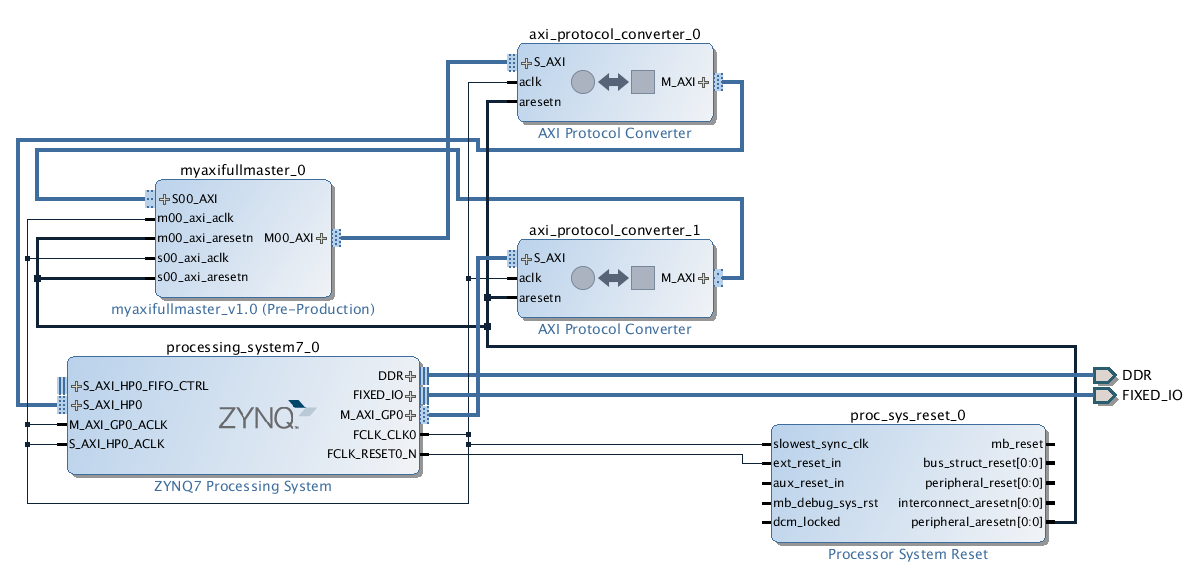
\includegraphics[width=\textwidth]{user_man_bloc_design}
	\caption{{\em Bloc design} d'un projet utilisant l'IP réseau de neurones}
	\label{fig:user_man_bloc_design}
\end{figure}

Pour modifier les paramètres et générer le bitstream, il faut se référer à la
partie~\ref{plan:user_man_modif_param}
page~\pageref{plan:user_man_modif_param}.


\subsubsection{Modifications des paramètres du réseau de neurones}
\label{plan:user_man_modif_param}

Pour modifier les paramètres du réseau de neurones (nombre de neurones de chaque
niveau et taille des images), il faut préciser à {\em Vivado} que les fichiers sources
de l'IP ont changés. Pour cela, il faut:
\begin{enumerate}
	\item modifier dans le fichier \verb+myaxifullmaster_v1_0_S00_AXI.vhd+ (situé dans le sous-dossier \verb+hdl/+ de  \verb+<dossier_contenant_les_IPs>/my_axi_full_master+), les paramètres~:
		\begin{itemize}
			\item \verb+LAYER1_FSIZE+ pour changer la taille des images en entrée
			\item \verb+LAYER1_NBNEU+ pour changer le nombre de neurones dans le premier niveau
			\item \verb+LAYER2_NBNEU+ pour changer le nombre de neurones dans le deuxième niveau
		\end{itemize}
	\item sélectionner l'IP dans la partie "{\em Project Manager}"
		et avec un clic-droit sélectionner l'option "{\em Re-package IP}".
		Dans la partie "{\em Review and package}", cliquer sur "{\em Re-package IP}" afin de confirmer
		les modifications des fichiers sources de l'IP et retourner sur la fenêtre principale de {\em Vivado}.
\end{enumerate}
~\\
Une fois cela fait, il faut générer le nouveau bitstream en cliquant sur "{\em Generate Bitstream}".
Après génération, il faut faire "{\em File-> export Hardware (cocher include bitstream) -> Ok}".
Enfin pour lancer {\em Xilinx SDK} afin de programmer le FPGA et lancer le logiciel embarqué, il faut faire "{\em File-> Launch SDK}".


%TODO: Partie SW et lancement de l'application

